\section{Overview}

This chapter describes the system design and presents the methodology
used to design and develop the project while achieving the objectives of
the study. It outlines the complete workflow of the project, starting
from the system concept and design requirements, through hardware and
firmware development, PCB design and manufacturing, and finally to
system deployment. The chapter also describes the calibration and
validation of the selected soil moisture sensor in comparison with
professional-class sensors.

\section{System Concept and Design
Requirements}

\subsection{System Concept}

The system is designed as a wireless mesh network using LoRa as the core
communication technology. Weatherproof wireless sensor nodes collect
data such as soil moisture, soil temperature, air humidity, and air
temperature, and transmit this data efficiently between neighboring
nodes until it reaches a base station with access to a cloud database.
The collected data is then made accessible to researchers from anywhere.

\begin{figure}[htbp]
\centering
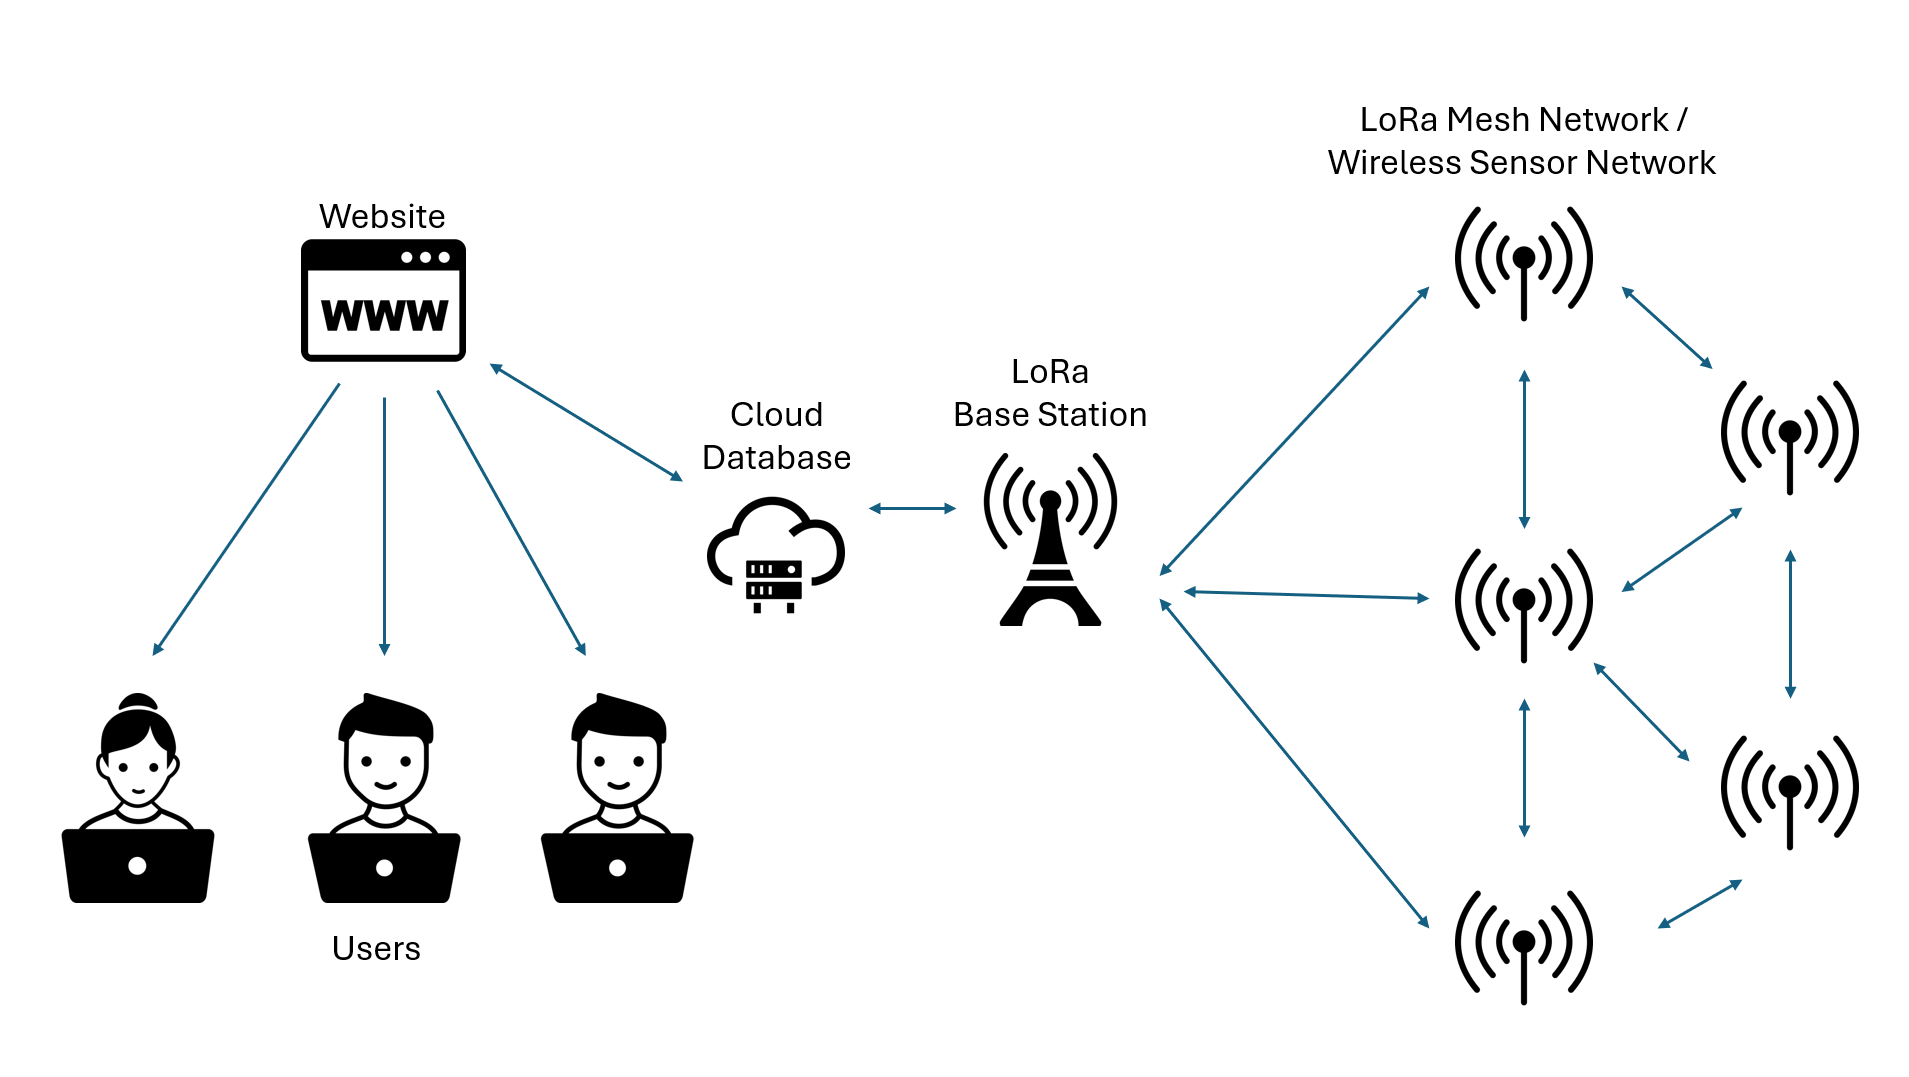
\includegraphics[width=5.03874in,height=2.8429in]{figs/method-image1.png}
\caption{System concept of the LoRa-based wireless sensor mesh network for monitoring turf roof conditions.}
\label{fig:smallcompile-system-concept}
\end{figure}

LoRa was selected for its effectiveness over the short to medium
distances between turf houses, with the mesh topology improving network
robustness.


\textbf{\hfill\break
}